% !TeX root = ../../latex-talk.tex

\part{像模像样 \LaTeX{}}

\section{TikZ}



\section{PGFPlots}

\begin{frame}
    \frametitle{PGFPlotsEdt 帮助我完成物理实验报告图...}
    \begin{columns}
        \begin{column}{0.25\textwidth}
            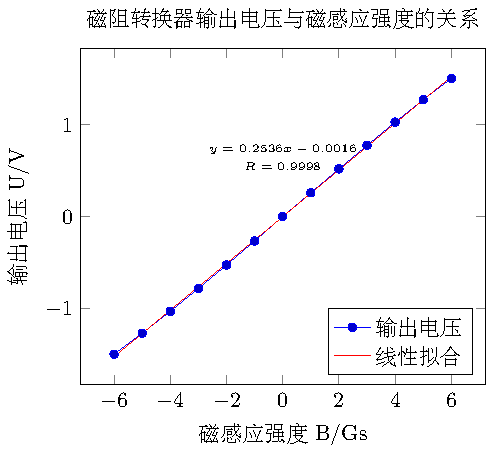
\includegraphics[width=\linewidth]{a}
            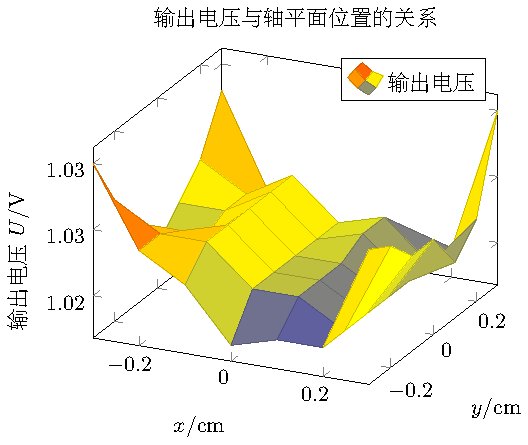
\includegraphics[width=\linewidth]{b}
        \end{column}
        \begin{column}{0.50\textwidth}
            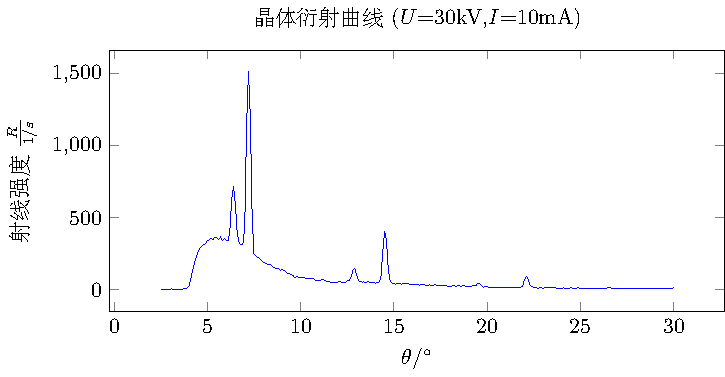
\includegraphics[width=\linewidth]{c}
            \begin{columns}
                \begin{column}{0.5\linewidth}
                    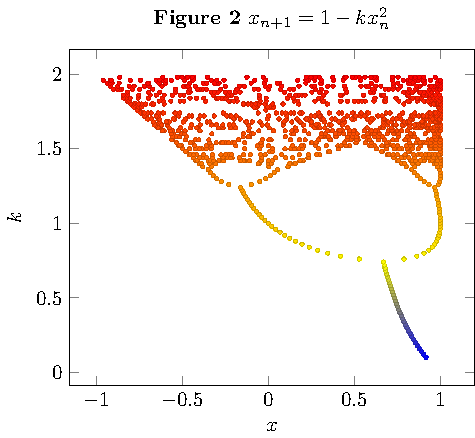
\includegraphics[width=\linewidth]{d}
                \end{column}
                \begin{column}{0.5\linewidth}
                    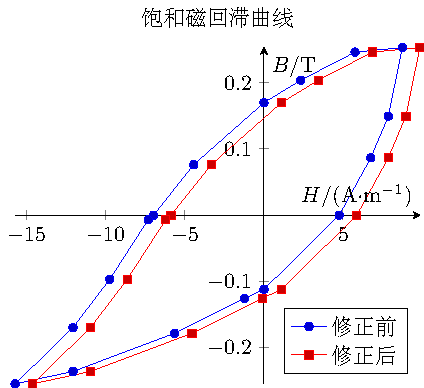
\includegraphics[width=\linewidth]{e}
                \end{column}
            \end{columns}
        \end{column}
        \begin{column}{0.25\textwidth}
            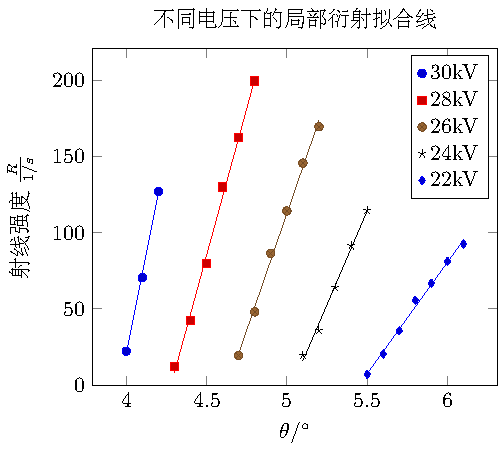
\includegraphics[width=\linewidth]{f}
            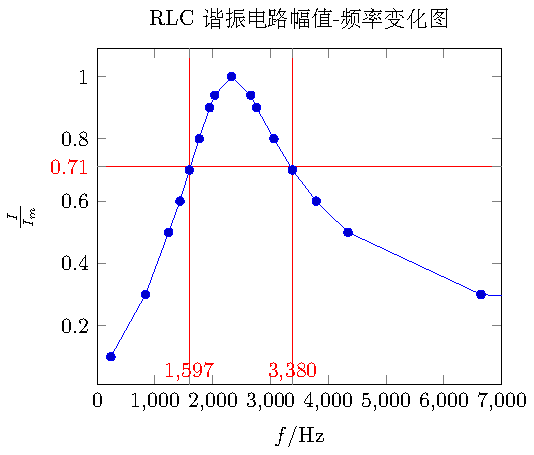
\includegraphics[width=\linewidth]{g}
        \end{column}
    \end{columns}
\end{frame}